\documentclass[sigconf,anonymous]{aamas}
\usepackage{balance}
\usepackage{booktabs}
\usepackage{amsmath}
\usepackage{graphicx}
\newcommand{\PrimaryRows}{%
Qwen3.6 & Base & 0.13132 & 0.13008 & $+0.00123$ $[-0.00053,+0.00363]$ & .022\\
Qwen3.6 & Wrong persona & 0.13132 & 0.17410 & $-0.04278$ $[-0.04781,-0.03696]$ & .022\\
Qwen3.6 & OPRO & 0.13132 & 0.13152 & $-0.00020$ $[-0.00143,+0.00083]$ & 1.000\\
Qwen3.6 & Ridge & 0.13132 & 0.10955 & $+0.02177$ $[+0.01974,+0.02417]$ & .022\\
Granite & Base & 0.13594 & 0.13656 & $-0.00063$ $[-0.00199,+0.00098]$ & .023\\
Granite & Wrong persona & 0.13594 & 0.16819 & $-0.03225$ $[-0.03572,-0.02824]$ & .022\\
Granite & Native GigaEvo & 0.13594 & 0.13670 & $-0.00076$ $[-0.00400,+0.00385]$ & .022\\
Granite & Ridge & 0.13594 & 0.10955 & $+0.02639$ $[+0.02455,+0.02834]$ & .022\\%
}

\newcommand{\AllRows}{%
GA & $+0.00118$ $[+0.00053,+0.00178]$ & .022 & $-0.00136$ $[-0.00206,-0.00074]$$^{\dagger}$ & .022\\
DE & $+0.00089$ $[-0.00007,+0.00201]$ & .022 & $-0.00116$ $[-0.00249,+0.00058]$ & .022\\
PromptBreeder & $+0.00246$ $[-0.00069,+0.00495]$ & .022 & $-0.00053$ $[-0.00235,+0.00251]$ & .023\\
MAP-Elites-style & $+0.00123$ $[-0.00053,+0.00363]$ & .022 & $-0.00063$ $[-0.00199,+0.00098]$ & .023\\
GEPA-style & $+0.00010$ $[-0.00151,+0.00145]$ & 1.000 & $-0.00087$ $[-0.00322,+0.00170]$ & .022\\
Official GEPA & $-0.00020$ $[-0.00122,+0.00101]$ & 1.000 & $-0.00045$ $[-0.00168,+0.00061]$ & .842\\
Native GigaEvo & $-0.00009$ $[-0.00130,+0.00104]$ & 1.000 & $+0.00014$ $[-0.00280,+0.00213]$ & 1.000\\
OPRO & $+0.00143$ $[-3.2\times10^{-6},+0.00308]$ & .022 & $+0.00074$ $[-0.00136,+0.00420]$ & .022\\
ProTeGi & $+0.00244$ $[+0.00101,+0.00405]$ & .022 & $-0.00250$ $[-0.00343,-0.00174]$$^{\dagger}$ & .022\\
Random & $+0.00086$ $[+0.00039,+0.00133]$ & .022 & $+0.00115$ $[-0.00128,+0.00444]$ & .022\\
Best-of-budget & $-0.00044$ $[-0.00112,+0.00020]$ & .272 & $-0.00171$ $[-0.00211,-0.00131]$$^{\dagger}$ & .022\\
\midrule
GA, calibrated fitness & $-0.00044$ $[-0.00104,+0.00016]$ & .582 & $-0.00266$ $[-0.00318,-0.00213]$$^{\dagger}$ & .022\\
GA, legacy fitness & $+0.00080$ $[+3.0\times10^{-7},+0.00164]$ & .022 & $-0.00166$ $[-0.00255,-0.00082]$$^{\dagger}$ & .022\\
MAP-Elites, calibrated fitness & $-0.00034$ $[-0.00099,+0.00030]$ & 1.000 & $-0.00267$ $[-0.00377,-0.00179]$$^{\dagger}$ & .022\\%
}

\newcommand{\SeedRows}{%
Qwen3.6 & GA, raw & 0.15665 & 0.13127 & +0.00132, +0.00134, +0.00087\\
Qwen3.6 & GA, calibrated & 0.16377 & 0.12965 & -0.00066, +0.00003, -0.00069\\
Qwen3.6 & MAP-Elites, raw & 0.15577 & 0.13132 & -0.00053, +0.00045, +0.00378\\
Qwen3.6 & MAP-Elites, calibrated & 0.17042 & 0.12976 & -0.00029, -0.00087, +0.00015\\
Granite & GA, raw & 0.17209 & 0.13520 & -0.00090, -0.00195, -0.00123\\
Granite & GA, calibrated & 0.18219 & 0.13391 & -0.00295, -0.00280, -0.00223\\
Granite & MAP-Elites, raw & 0.17640 & 0.13594 & -0.00202, -0.00096, +0.00110\\
Granite & MAP-Elites, calibrated & 0.18436 & 0.13389 & -0.00203, -0.00385, -0.00214\\%
}


% Official AAMAS 2027 template, downloaded from the conference website.
\makeatletter
\gdef\@copyrightpermission{
  \begin{minipage}{0.2\columnwidth}
   \href{https://creativecommons.org/licenses/by/4.0/}{
\includegraphics[width=0.90\textwidth]{by}}
  \end{minipage}\hfill
  \begin{minipage}{0.8\columnwidth}
   \href{https://creativecommons.org/licenses/by/4.0/}{This work is licensed under a Creative Commons Attribution International 4.0 License.}
  \end{minipage}
  \vspace{5pt}
}
\makeatother
\setcopyright{ifaamas}
\acmConference[AAMAS 2027]{Proc.\@ of the 26th International Conference
on Autonomous Agents and Multiagent Systems (AAMAS 2027)}{3--7 May 2027}{Hanoi, Vietnam}{M.~Baldoni, F.~Fang, W.~Yeoh, N.~Yorke-Smith (eds.)}
\copyrightyear{2027}
\acmYear{2027}
\acmDOI{}
\acmISBN{}
\acmSubmissionID{TBD}
\submissionType{Research Paper Track}
\title[Predictive Personas]{Do Optimized Personas Predict New Respondents?}

% No author names or affiliations in the anonymous submission.

\begin{abstract}
Can optimized language-model personas predict a new person's answers from a
limited response history? A fixed Granite calibrated-GA persona mixed with
ridge fitted on 80 paired people improves ranked probability score (RPS;
lower is better) over both neutral-persona mixture controls on a third,
inventoried-disjoint panel of 600 respondents from the same corpus. Across
categorical and raw-history representations, the four gains are
0.00125--0.00184 RPS, with positive paired 95\% intervals and Holm-adjusted
$p=.0008$. The old prompts, calibration, ridge fits and mixture weights were
fixed before these respondents' target answers were scored; uncertainty
conditions on three old search seeds and three fixed ridge subsets.
This is restricted utility of a prompt-plus-weight recipe, not a prompt-only
effect or an equal-total-supervision comparison. The full 8,000-person
same-history ridge remains much stronger. In our original 84-template,
two-model comparison, the planned raw-fitness MAP-Elites-style method does
not establish improvement over its neutral base or strongest search rival.
On a separate additional 600, two Granite templates beat neutral, but their
declared MAP calibrated-versus-raw contrast fails its interval rule; Qwen
neutral comparisons remain null. A same-shortlist selector changes 11 of 12
winners on the exposed original cohort without a clear final-score benefit.
These findings delimit a useful old-recipe regime, not a new optimizer,
new-search reliability, external behavioral validity or superiority to ridge
with full training data.
\end{abstract}
\ccsdesc[500]{Computing methodologies~Intelligent agents}
\ccsdesc[300]{Computing methodologies~Machine learning}
\keywords{human simulation, language-model agents, prompt optimization,
proper scoring rules, respondent prediction}
\begin{document}
\maketitle

\section{Introduction}
An agent that answers a questionnaire in character is useful as an individual
predictor only if its answers forecast a particular unseen person better than
simpler uses of the same human information. Population-level resemblance,
plausible prose, and a high score on people used for prompt selection do not
establish that property. This is a practical issue for survey simulation,
where the relevant unit of analysis is the individual and acquiring
respondent-level self-reports entails time and compensation costs~\cite{park2026selfreports}.
Prior work on personality-conditioned agents evaluates induced behavioral
style through changes in task selection~\cite{newsham2025personality}; our
target is the human associated with a profile.

We study a reusable \emph{persona template}: a prompt optimized on development
respondents, then instantiated from a new respondent's 60 observed answers
to forecast 60 different answers. The template cannot use that person's target
answers, target-derived cluster, or evaluation outcomes. We ask whether
proper-score search improves predictions under this restriction and whether
any improvement exceeds budget-matched search and statistical predictors
with access to the same observed items.

We address three questions. \textbf{RQ1:} Does the planned primary search
method improve held-out predictions over base and the strongest search
comparator chosen on development data? \textbf{RQ2:} Does changing the fitness
objective improve the final calibrated score? \textbf{RQ3:} Does matching a
persona to its respondent carry predictive information, and how does that
information compare with a statistical predictor using the same history?

We contribute a frozen comparison of reusable persona search and an empirical
map of the prediction choices it supports. Its clearest positive result is
restricted incremental utility: the old Granite calibrated-GA persona plus
ordinary ridge, with the old selected weight, beats both matched neutral
mixtures on a third same-corpus respondent panel when the ridge fit uses 80
paired people. That fit budget does not count all search, selection,
calibration, population-prior, and per-person observed-answer supervision.
Proper-score calibration changes
the search landscape: across 24 saved pools, median raw versus calibrated
candidate-rank discordance is 35.6\%. The original Granite MAP-Elites-style
contrast and additional GA contrasts favor calibrated fitness in three
observed runs. A separate additional-respondent test of historical frozen
templates supports two Granite gains over neutral, but its declared MAP-Elites
objective contrast does not pass the combined rule. The exact categorical
profile supplied to the LLM is itself a strong predictive representation:
ridge fitted on 8,000 people retains 89.8\% of the raw-history predictor's
improvement over the prior and remains stronger on additional respondents.
Adaptive label-budget and mixture diagnostics on the exposed original cohort
are exploratory. The new-panel mixture comparison tests the old selected
recipe, conditional on its three historical search seeds, and does not imply
cross-model optimized-prompt necessity. Answer equivalents provide a secondary
effect-size translation.

The practical question is incremental predictive value beyond structured
history. Our controls separate profile matching from that deployment benefit.

\section{Related work}\label{sec:related}
\paragraph{Personality and agent behavior.}
Newsham and Prince~\cite{newsham2025personality} study how induced OCEAN
traits alter task selection by LLM agents. Xu et al.~\cite{xu2023dialogues}
condition narrative dialogue on personality representations and evaluate it
with automatic measures and human judgments. These studies ask whether an
agent expresses a supplied personality. Our outcome is a probability forecast
for a particular held-out human, so trait expression alone cannot validate it.
Jahan and Mell~\cite{jahan2024negotiation} relate personality and self-reports
to behavior in human--agent negotiation. That behavioral criterion is distinct
from our questionnaire target: our results do not establish transfer to
negotiation or other interactive decisions.

\paragraph{Individual prediction and prompt search.}
Persona-based simulation~\cite{hu2024persona,park2026selfreports} and learned
models of human cognition~\cite{binz2025centaur} motivate evaluating human
outcomes directly. We isolate a narrower intervention: changing reusable
persona instructions while fixing the observed items and readout model.
Hu and Collier compare persona prediction with supervised linear regression.
We extend that comparison to fitting budget, exact rendered features and
search-objective choice. Recent work tests temporal prediction~\cite{jia2026reliably}
and attribute-dependent population alignment~\cite{frohling2026attributes};
we isolate prompt optimization within one inventory. Aher et al.~\cite{aher2023simulation} instead evaluate
replication of human-subject study patterns; our target is each held-out
respondent's disjoint questionnaire answers.
Argyle et al.~\cite{argyle2023samples} study demographic conditioning of
synthetic survey samples. Bisbee et al.~\cite{bisbee2024synthetic} find that
similar survey means can coexist with distorted variation and associations;
Tjuatja et al.~\cite{tjuatja2024biases} show that survey response biases often
differ between LLMs and humans. We therefore test matched individual forecasts,
without treating predictive gains as validation of human-like behavior.
Our search families draw on EvoPrompt~\cite{guo2024connecting},
PromptBreeder~\cite{fernando2024promptbreeder}, OPRO~\cite{yang2024opro},
ProTeGi~\cite{pryzant2023protegi}, and GEPA~\cite{agrawal2025gepa}. Calibration-aware
selection also appears in Reflective Prompt Tuning~\cite{bayat2026reflective}; we test objective
effects under fixed information and budget.

Unlike MADRID's adversarial-scenario search~\cite{mouret2015mapping,samvelyan2024madrid},
we optimize individual response forecasts.

\section{Task and method}\label{sec:task}
Figure~\ref{fig:pipeline} separates the per-person forecast from the
development, freezing and evaluation stages.
\begin{figure*}[t]
\centering
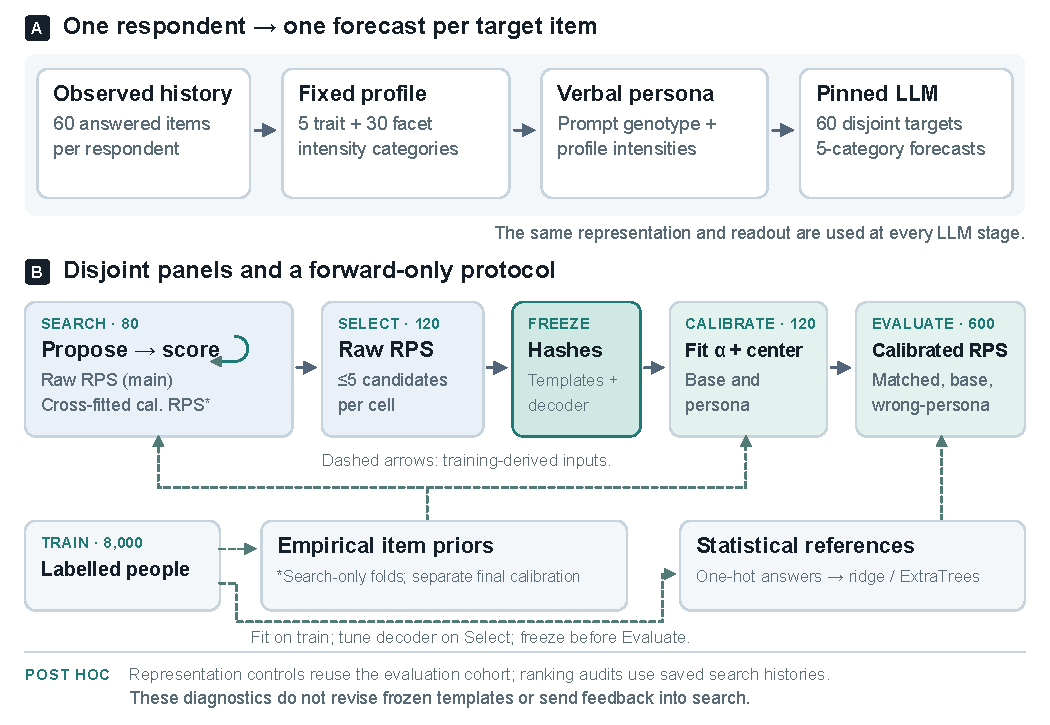
\includegraphics[width=\textwidth]{figure_pipeline.pdf}
\Description{Respondent representation above a search, raw selection, freeze,
calibration and evaluation protocol. Training supplies item priors and
statistical references. Post-hoc diagnostics are separate.}
\caption{Persona forecasting and frozen evaluation. (A) Sixty observed answers
become 35 categorical profile values; searched wording and a pinned readout
produce ordinal forecasts for 60 disjoint items. (B) Respondent panels are
disjoint. Search uses raw or cross-fitted calibrated RPS, but every shortlist
is selected by raw RPS. Templates and decoder choices are frozen before final
calibration and evaluation. Dashed arrows show training-derived inputs.
Post-hoc diagnostics do not revise templates or feed back into search.
The legacy GA fitness control is omitted for readability.}
\label{fig:pipeline}
\end{figure*}
\subsection{Respondent forecasting}
Let $x_i$ be a new respondent's answers to the fixed 60 input items and
$y_{ij}\in\{1,\ldots,5\}$ the answer to target item $j$ from the disjoint
60-item set. A frozen template $g$ constructs a persona $g(x_i)$, and a pinned
readout model returns an ordinal distribution $p_{ij}(k)$. We evaluate the
normalized ranked probability score (RPS), a proper scoring
rule for ordinal forecasts~\cite{gneiting2007proper}
\begin{equation}
 \mathrm{RPS}(p,y)=\frac{1}{K-1}\sum_{k=1}^{K-1}
 \left(\sum_{h=1}^{k}p(h)-\mathbf 1\{y\leq k\}\right)^2,\quad K=5.
\end{equation}
Lower is better. We average the 60 target-item losses within each respondent
before averaging respondents; a search seed is a repeated optimization run,
not a new person. Our primary estimand is the respondent-population mean paired change in
calibrated RPS, averaged over the three frozen search runs. Inference over
fresh optimizer runs is a separate target.
We retain five-category probability estimates and digit-token mass so that
losses and readout coverage can be checked separately.

\subsection{Information available to the persona}
The IPIP-NEO-120 inventory measures 30 facets of five personality
traits~\cite{johnson2014ipip}. The renderer converts the observed input items
into facet means on a 0--100 scale, averages facets within each trait, and
maps these scores to fixed verbal intensity modifiers. A template supplies
a role definition, five trait formulations, 30 facet formulations, and an
internal-reflection instruction. Search edits these text fields; the
intensity mapping and item split are fixed. The neutral base uses the same
renderer with standard construct names and instructions to answer from the
supplied profile. No target-derived cluster selects a template.

Thus the LLM receives a compressed verbal profile, not a transcript of all
60 answers. All LLM search arms share this representation. The statistical
reference receives the same observed items as one-hot encoded answers.
This matches available human history but does not match representation:
any LLM--ridge gap combines the effects of compression, readout, and learning.
We therefore add a post-hoc predictor fitted to the exact categorical profile
to determine whether compression alone can explain that gap. The comparison
still differs in fitted predictor and training objective, so it cannot isolate
an intrinsic limitation of the LLM architecture.

\subsection{Readout and calibration}\label{sec:calibration}
Each target is presented with a five-point response scale using the model's
chat template and the assistant prefill \texttt{My answer is}. The readout
requests one token at temperature zero with top-20 log probabilities. It sums
the returned probabilities for answer digits 1--5 and normalizes their mass;
if their total mass is zero, the implemented fallback is uniform. These are
estimates derived from returned digit probabilities, not exact full-vocabulary
probabilities. Reverse-keyed items are mapped onto the corpus's recoded scale
before scoring. Digit mass and the fraction below 0.5 are retained separately.

Let $Q_{ij}$ denote the model's four-threshold CDF, $F_{0j}$ the empirical
CDF from training respondents, and $\bar Q_j^{C}$ the mean model CDF on the
calibration panel. The evaluated forecast is
\begin{equation}
 \widetilde Q_{ij}=\Pi_{\mathcal C}
 \left[F_{0j}+\alpha\left(Q_{ij}-\bar Q_j^{C}\right)\right],
 \label{eq:calibration}
\end{equation}
where $\Pi_{\mathcal C}$ minimizes squared error over CDFs bounded by 0 and 1.
For each selected template and the base, $\alpha$ minimizes calibration-panel
RPS over $\{0,.1,\ldots,1,1.2,1.4,1.6,1.8,2\}$. The resulting $\alpha$ and
centering vector are then fixed on evaluation respondents. Wrong-persona
forecasts use the evolved template's calibration parameters unchanged.
The training labels therefore contribute to LLM calibration as well as to
the statistical references; this is a target-supervised evaluation.

The main search objective is \emph{raw} RPS. In calibrated-fitness controls,
$\alpha$ and the centering vector are fitted on one fixed half of the search
panel and scored on the other half, then swapped. These two folds are shared
across candidates and seeds. The final calibration panel is not used during
search. All variants still use raw RPS for shortlist selection. The legacy
GA control minimizes the negative expected proximity
$-\left[1-\sum_{k=1}^{5}p(k)|k-y|/4\right]$, rather than RPS.

\subsection{Persona search}\label{sec:search}
The two readout families are Qwen3.6-35B-A3B and Granite-4.2-30B; a pinned
Qwen3.8-27B mutator proposes edits. The eleven methods are GA, DE,
PromptBreeder, MAP-Elites-style search, GEPA-style search, official GEPA,
native GigaEvo, OPRO, ProTeGi, random search, and best-of-budget.
GA and DE adapt EvoPrompt's evolutionary operators to the common JSON
schema. PromptBreeder evolves mutation instructions; OPRO uses scored
history; ProTeGi uses textual critiques. Random search independently mutates
the seed template, while best-of-budget samples initial candidates without
an evolutionary trajectory. Local adapters share the task-specific genotype,
feedback, and evaluator; they are not replications of the original papers'
benchmark results. Official GEPA v0.1.4 and native GigaEvo v2.20.1 are
pinned separately from their local style-based counterparts.

The MAP-Elites-style adapter uses two islands and an archive indexed by
prompt length and predicted-response standard deviation. It starts with four
candidates per island and mutates candidates until the forecast budget is
exhausted, with migration every 12 iterations and a six-observation insight
window. These are fixed search settings, not evidence that archive diversity
causes an improvement. The GA also stops on the forecast budget; its settings
are population eight, two elites, tournament
size three, crossover probability 0.8, and mutation probability 0.3.
The common genotype-proposal settings are temperature 0.7 and a 2,500-token
output cap; auxiliary operator requests can use different settings.

One full-panel forecast equivalent is $80\times60=4{,}800$ respondent--item
forecasts. Each cell is capped at 80 equivalents, or 384,000 executed
candidate forecasts; fractional evaluations consume their actual share.
Shortlist selection has a separate cap of five candidates on 120 people.
Failed proposals and their available token costs are retained separately;
a proposal is not credited with forecasts that did not occur. Equal forecast
caps do not imply equal tokens, mutator calls, or wall time.

\section{Experimental design}\label{sec:controls}
\subsection{Splits, freezing, and controls}
We use the complete-case IPIP-NEO-120 corpus with split seed 20261004.
A source audit matches all 410,168 retained records to the original archive
by respondent ID and item values (Supplementary Material). Table~\ref{tab:splits} gives respondent roles. Previously
used historical IDs, saved response fingerprints, and baseline-panel IDs are
excluded according to the available exposure inventory. This reduces
within-program exposure but does not establish that the public corpus was
absent from model pretraining or earlier methodological development.

\begin{table}[t]
\caption{Fixed respondent roles. IDs are disjoint across rows; the 60 observed
items and 60 target items are disjoint within every row.}
\label{tab:splits}\centering\small
\begin{tabular}{@{}lrl@{}}\toprule
Split & People & Permitted use\\\midrule
Train & 8,000 & Priors and statistical fitting\\
Search & 80 & Candidate fitness\\
Select & 120 & Prompt and decoder selection\\
Calibrate & 120 & Final LLM calibration\\
Evaluate & 600 & Frozen comparison\\\bottomrule
\end{tabular}
\end{table}

The design has 66 main cells (11 methods, two models, seeds 1--3) and 18
additional cells (GA with calibrated or legacy fitness and MAP-Elites-style
search with calibrated fitness). The fixed manifest names raw-fitness
MAP-Elites-style search as primary. Within each model, the lowest mean
selection-panel raw RPS across seeds chooses the strongest non-primary search
comparator, excluding objective variants. This yields OPRO for Qwen3.6 and
native GigaEvo for Granite. The 84 selected templates and the statistical
decoder configuration are hash-bound before final evaluation. These are
internal protocol and freeze records, not an assertion of external
preregistration.

Every final cell evaluates the frozen template and neutral base on the same
600 people. Base forecasts are recomputed in each cell; the base score in a
paired comparison is the corresponding cell's score, not a pooled reference
from another run. A common derangement assigns another person's profile to
each respondent, with no fixed points. It retains the target item and model,
measuring whether matching the profile to the respondent matters.

The statistical controls are an empirical item prior, a multioutput ridge
ordinal-CDF predictor, and ExtraTrees. Both learned references use one-hot
encoding of the 60 observed answers and are fitted on the 8,000 training
people. Ridge selects its penalty from $\{1,10,100,1000\}$; ExtraTrees uses
64 trees and chooses minimum leaf size from $\{10,30\}$. Selection-panel RPS
chooses hyperparameters and the strongest family (ridge). Unlike LLM readouts,
these references use no calibration targets; the comparison matches input
history, not total supervision. Evaluation people fit neither predictor.
Predicted CDFs are projected onto valid ordinal distributions before scoring.

Retained-information curves use ridge, three frozen nested input orders,
and budgets $m\in\{0,1,2,5,10,20,30,40,60\}$. Ridge is tuned separately at
each positive budget. Monotonic regression and interpolation translate the
persona loss into an answer equivalent. This is information retained under
a specified decoder, not the number of questionnaire answers literally saved.

\subsection{Uncertainty and decision rule}
The unit of inference is a respondent from the filtered corpus, with the same
people paired across methods and seeds. Estimates condition on archived readouts. For losses $L_{is}^{A}$ and $L_{is}^{B}$, the estimated
contrast is $\widehat\Delta=N^{-1}\sum_i[3^{-1}\sum_{s=1}^{3}
(L_{is}^{A}-L_{is}^{B})]$. Raw and calibrated runs are paired by initialization
seed index and share respondent panels and calibration folds. Their adaptive
search paths differ; this pairing does not ensure identical mutator samples
or serving execution. We use 5,000 crossed bootstrap draws resampling both
respondents and the three search seeds, and 5,000 two-sided respondent-level
sign flips after averaging the three seeds. The sign-flip test conditions on the three frozen runs; the crossed interval
additionally describes sensitivity to resampling those observed runs, not
validated uncertainty for new optimizer runs. Thus a
small conditional $p$ value can accompany a crossed interval containing zero. Holm correction covers all 110 comparisons in the
analysis: 84 arm-versus-base/decoder/wrong-persona contrasts and 26
primary-versus-other-arm contrasts across the two models. Displaying a subset
does not change that correction family. At this simulation resolution,
several adjusted values equal approximately .022; they are not precise
estimates of identical underlying probabilities.

We require a crossed interval excluding zero in the favorable direction and
an adjusted $p<.05$ before describing a contrast as an improvement. These are
different uncertainty calculations, not an interval and test obtained by
inverting the same procedure. A benefit relative to base is distinct from
practical superiority to the strongest same-history statistical reference.
A missing final prediction fails a cell instead of dropping a difficult
respondent. Hash checks enforce a common panel, manifest, selected templates,
and decoder before combining results.

\subsection{Additional-respondent fixed-template transfer}
After inspecting the original cohort, we fixed a separate test of 24 historical
GA and MAP-Elites-style winners (two models, raw or calibrated fitness, three
old seeds) on 600 additional people from the same IPIP120 corpus. The new IDs
were sampled from 36,119 complete eligible cases after excluding the reachable
inventoried historical exposure union; unknown lifetime and pretraining
exposure remain possible. Original Train8000 priors, Calibrate120 weights and
CDF centers, model snapshots, selected templates, and ridge specification
were retained. No new prompt search or selector intervention was run. The
internally frozen primary family comprises three Granite contrasts:
calibrated versus raw MAP-Elites-style winners, calibrated MAP-Elites-style
versus its neutral base, and calibrated GA versus its neutral base. We apply
the same favorable crossed-interval and Holm-$p<.05$ rule, correcting the
three sign-flip tests together. Qwen, wrong-profile, same-history ridge, and
other arm contrasts are reported as diagnostics. The supplemental protocol
and full results separate this test from the original 110-comparison family.

\subsection{Exploratory same-shortlist selector study}
After inspecting the original evaluation, we re-scored the same five archived
candidates in each of 12 GA searches (two models, raw/calibrated search
fitness, three old seeds) on the original Select120. Fresh forecasts gave
both a raw-RPS and a two-fold cross-fitted calibrated-RPS selector per pool;
all winner identities were frozen before re-evaluating them, with fresh
neutral bases, on the \emph{already exposed} original Evaluate600. Each
winner refits calibration on the original Calibrate120. Four direct selector
effects, four search-objective effects and two interactions form a separate
ten-test, two-sided Holm family. Crossed intervals resample respondents and
the three observed seeds; sign flips condition on those archived runs. This
study neither supplies new people nor tests new search trajectories or E1's
additional respondents (Supplementary Material).

\subsection{Frozen Granite-80 mixture transfer}
After inspecting the original, additional-respondent, and selector outcomes,
we internally froze a narrower test on a third 600-person panel from the same
IPIP120 corpus. Its IDs exclude every original split, the first additional
panel, and the reachable historical exposure inventory. Only IDs and item
missingness determined eligibility; target answers were opened after the old
recipe and panel were frozen. We reused the three historical Granite
calibrated-GA prompts, their neutral counterparts, old calibration and
population prior, and six ordinary and six prior-anchored ridge fits for
categorical/raw representations and three disjoint 80-person training
subsets. Old Calibrate120 was split into 60 calibration people and 60 people
for independent mixture-weight selection. Ridge penalties used old Select120.
The 80 people are a paired \emph{ridge fitting} budget, not total target-label
supervision: search, selection, prior, calibration and each new person's 60
observed answers also contribute information.

For each representation, we compare the optimized persona plus ordinary ridge with neutral persona plus (i) the strongest prior-anchored ridge and
(ii) the same ordinary ridge. The neutral arms retain their own previously
selected weights. Thus (ii) holds ridge coefficients fixed but tests the
optimized prompt-plus-weight recipe, not a prompt-only intervention. The four
comparator-minus-hybrid RPS contrasts form one two-sided Holm family. We
average nine fixed per-person \emph{loss} vectors (three old search seeds by
three fixed ridge subsets) before paired respondent inference. A
representation passes only if both gains are at least 0.001 RPS, both paired
95\% bootstrap lower bounds exceed zero and both adjusted respondent
sign-flip $p$ values are below .05. Intervals condition on those old fits and
this panel; they do not quantify new optimizer-run variability. The protocol,
full controls and source lineage are in the Supplementary Material.

\paragraph{Fixed-weight readback.}
After E3 outcomes were inspected, we froze a CPU-only analysis of its
\emph{exposed} 600-person panel. For each representation we reuse the same
ordinary ridge and set persona weight to 0.5 for both optimized and neutral
forecasts, retaining each arm's historical calibration. Two paired
neutral-minus-optimized RPS effects form a separate Holm family. We average
the nine fixed per-person losses before respondent-level inference. This
compares calibrated forecast packages at equal weight, not prompt text alone
or new respondents. A fixed five-weight grid, three old-seed and
leave-one-old-seed-out summaries, and uncalibrated forecasts are descriptive
diagnostics (Supplementary Material).

\subsection{Additional diagnostic protocol}\label{sec:diagnostic}
Saved-forecast diagnostics on the already exposed original cohort are post
hoc. Separate Holm families cover 33 representation contrasts, nine objective
contrasts and 48 contrasts per fitting-budget or mixture screen; they do not
replace the original 110-test family. Linear CDF pooling follows
$H=(1-w)R+wP$~\cite{gneiting2011combining}. Original Cal120 separates
60-person persona calibration from 60-person mixture selection; each rival
selects its own weight. Training subsets overlap, and intervals condition on
fixed statistical fits and old search seeds. The supplement gives features,
penalty/weight grids, all budgets, controls and full exposure history.

\section{Results}\label{sec:results}
\subsection{Coverage and scoring verification}
All 84 frozen final cells completed, each with 600 respondents and 36,000
observed target answers. Final receipts contain no failed requests or
uncertain forecasts. They record 10,281,600 confirmed forecasts and
11,979,632,160 prompt tokens. Per cell, the count is
$2(120)(60)+3(600)(60)=122{,}400$: calibration forecasts for base and evolved
personas plus evaluation forecasts for base, evolved, and wrong personas.
These totals concern the final stage, not search or total project cost.

A separate raw-prediction audit reloaded all 84 saved probability files and
original item labels, selected calibration weights anew from saved calibration
predictions, and reproduced each base, evolved, and wrong-persona
per-respondent loss to absolute tolerance $10^{-10}$. This validates the saved
scoring computation; it does not independently replay model inference or the
full search trajectories.

\subsection{RQ1: Primary search and the full comparison}
Table~\ref{tab:main} reports the planned primary contrasts. The raw-fitness
MAP-Elites-style method has no crossed interval wholly below zero against
base on either model. Nor does it establish an advantage over OPRO on Qwen
or native GigaEvo on Granite. These are inconclusive superiority comparisons,
not evidence of equivalence.

\begin{table*}[t]
\caption{Planned primary comparisons. $\Delta$ is raw-fitness MAP-Elites-style
persona minus control in calibrated RPS (lower is better). Crossed 95\%
intervals resample respondents and search seeds; Holm-adjusted sign-flip
$p$ values condition on the three observed seeds. All rows use the same 600
people. Small discrepancies between rounded means and differences arise
because differences are computed before rounding.}
\label{tab:main}\centering\small
\begin{tabular}{@{}llrrll@{}}\toprule
Model & Control & Persona RPS & Control RPS & $\Delta$RPS [95\% CI] & $p_{\mathrm H}$\\\midrule
\PrimaryRows
\bottomrule\end{tabular}
\end{table*}

Table~\ref{tab:all} gives all 14 method--objective identities, including
unfavorable and inconclusive outcomes. None improves over base under the
stated rule on \emph{both} models. Granite nevertheless has several
base-beating methods: raw and calibrated GA, legacy-fitness GA, calibrated
MAP-Elites-style search, ProTeGi, and best-of-budget. In particular, ProTeGi
improves by 0.00250 and best-of-budget by 0.00171 RPS. A favorable base
comparison therefore does not uniquely support evolutionary search or an
archive mechanism. We do not select a new primary method from this table.

\begin{table*}[t]
\caption{Complete method comparison: calibrated RPS difference from each
cell's base, with crossed 95\% intervals and respondent sign-flip Holm $p$
values conditional on three fixed runs, from the same 110-test family.
A dagger marks an interval wholly below zero and
$p_{\mathrm H}<.05$. The first eleven rows use raw-RPS fitness; the final
three are objective variants. Each entry aggregates three search seeds and
600 paired respondents.}
\label{tab:all}\centering\small
\begin{tabular}{@{}lllll@{}}\toprule
& \multicolumn{2}{c}{Qwen3.6} & \multicolumn{2}{c}{Granite}\\
Method & $\Delta$RPS [95\% CI] & $p_{\mathrm H}$ & $\Delta$RPS [95\% CI] & $p_{\mathrm H}$\\\midrule
\AllRows
\bottomrule\end{tabular}
\end{table*}

\subsection{RQ2: Fitness-objective effects}
The planned direct objective contrast for MAP-Elites-style search favors
calibrated fitness on Granite: raw minus calibrated RPS is 0.00205
(crossed interval $[0.00015,0.00340]$, Holm $p=.022$). Calibrated
MAP-Elites-style search is also 0.00267 below base, and calibrated GA is
0.00266 below base. Both calibrated variants improve over their corresponding
bases in all three observed Granite search seeds (Supplementary Material).
Their Qwen intervals versus base cross zero. This differs from the direct
objective effect: an objective can improve an otherwise harmful search without
establishing a benefit over the neutral profile.

The additional direct GA analysis finds raw-minus-calibrated effects of
0.00163 on Qwen (crossed interval $[0.00111,0.00219]$) and 0.00130 on
Granite ($[0.00060,0.00204]$). Each is positive in all three observed seeds
and has conditional Holm $p=.002$ in the new nine-test family.
The supplementary objective plot shows all four contrasts, including the
Qwen MAP-Elites seed with an unfavorable effect. All five interaction
intervals cross zero: significance in one subgroup and not another does not
demonstrate an interaction. The same MAP-Elites Granite contrast has $p=.022$
in the original 110-test family and $p=.002$ in the additional nine-test
family; the smaller value reflects a family change, not new evidence.





Candidate rankings reveal why raw RPS is not interchangeable with the
calibrated objective. Across the 24 search pools, median Spearman correlation
is 0.344 (range $-0.562$ to 0.788), median pairwise discordance is 35.6\%
(20.7--67.4\%), and median top-five overlap is zero (range 0--4). Thus
calibration changes candidate ordering, not only a score's scale. This is a
descriptive search-panel result; it does not prove that ranking changes
caused held-out gains. Final raw-RPS shortlist selection remains unchanged.

\subsection{Additional-respondent transfer of frozen templates}
All 24 fixed-template cells completed on the additional 600 respondents;
source, attempt, panel, probability, cost, and serving-log checks passed.
An independent CPU readback reproduced all saved losses and 16 reported
contrasts from raw forecasts (maximum absolute difference $8.33\times10^{-17}$).
In the declared Granite three-test family, calibrated MAP-Elites-style and GA
templates beat their respective neutral bases by 0.00216 RPS (crossed 95\%
interval $[0.00134,0.00311]$) and 0.00229 ($[0.00166,0.00289]$); both have
Holm-adjusted sign-flip $p=.0006$. The calibrated-versus-raw MAP-Elites-style
effect is $+0.00152$ raw minus calibrated, but its crossed interval
$[-0.00018,0.00273]$ includes zero, so it \emph{does not} pass the combined
rule despite adjusted $p=.0006$ and two favorable seed effects. This is
partial fixed-template transfer, not a replication of that objective effect
under the declared rule (full table in Supplementary Material).

Qwen calibrated GA and MAP-Elites-style winners beat their raw-fitness
counterparts by 0.00181 and 0.00168 RPS in diagnostic contrasts, but neither
beats its neutral base under the interval rule; both intervals include zero
(full diagnostic estimates in the supplement). The same-history
ridge scores 0.10821 on these people, against 0.12906/0.12920 for calibrated
Qwen GA/MAP and 0.13340/0.13353 for calibrated Granite GA/MAP. Thus the
positive Granite base comparisons do not establish practical superiority to
the stronger statistical control. Historical winners, old calibration and
three old search seeds were fixed; the test neither evaluates new search
trajectories nor the developmental aligned-selector winners.

\subsection{Exploratory selector intervention}
Fresh same-shortlist scoring changed 11 of 12 GA winners. Effects below
are calibrated minus raw selector RPS; negative favors calibration.
For Qwen calibrated search the effect is $-0.000153$, with crossed 95\%
interval $[-0.00050,0.00018]$; for raw search it is $-0.000587$,
with interval $[-0.00146,0.00004]$.
For Granite calibrated search the effect is $-0.000013$, with interval
$[-0.00021,0.00030]$; for raw search it is $-0.000473$, with interval
$[-0.00133,0.00010]$.
All four intervals include zero,
despite adjusted sign-flip $p=.0020$ for the two raw-search effects. Thus
substantial winner turnover does not establish final-score benefit under our
combined rule. The sole search-objective effect with an interval below zero
is Qwen calibrated versus raw search under the \emph{raw} selector; it does
not show a calibrated-selector gain. The supplementary ten-test table gives
all seed effects and adjusted probabilities.

\subsection{Frozen Granite-80 mixture transfer}
The third panel's four declared comparisons all pass the fixed rule
(Table~\ref{tab:e3}). The optimized mixture scores 0.13236 RPS with categorical
features and 0.13153 with raw history. The corresponding neutral mixtures
score 0.13382/0.13420 and 0.13278/0.13328, respectively. These are modest
gains for this old Granite recipe, conditional on nine fixed combinations;
they do not identify the isolated effect of changing a prompt. The full
8,000-person same-history ridge scores 0.10995 and remains substantially
better than either hybrid. All 216,000 new forecasts were confirmed; an
independent CPU recomputation agreed with saved losses and statistics within
$9.38\times10^{-11}$, below the fixed $10^{-10}$ tolerance. Individual
combination results, components, weights, exposure limits and costs appear in
the supplement.

\begin{table}[t]\centering\scriptsize
\caption{Third-panel Granite-80 old-recipe transfer. Positive gain is
comparator minus optimized hybrid RPS; paired intervals condition on nine
fixed old combinations. All four Holm-adjusted $p=.0008$. N=600.}
\label{tab:e3}
\begin{tabular}{@{}llr@{}}\toprule
Features & Neutral comparator & Gain [paired 95\% CI]\\\midrule
Categorical & Prior-anchored & $0.001465$ [$0.001213,0.001722$]\\
Categorical & Same ordinary ridge & $0.001843$ [$0.001595,0.002088$]\\
Raw & Prior-anchored & $0.001251$ [$0.001016,0.001490$]\\
Raw & Same ordinary ridge & $0.001747$ [$0.001519,0.001974$]\\\bottomrule
\end{tabular}\end{table}

\paragraph{Equal-weight diagnostic on the exposed E3 panel.}
At weight 0.5 with the same ordinary ridge, the old calibrated optimized
forecast package beats its neutral counterpart by 0.001477 RPS for
categorical features (paired 95\% CI $[0.001291,0.001676]$) and 0.001448
for raw history ($[0.001264,0.001643]$); both Holm-adjusted $p=.0004$.
All three historical-seed and all leave-one-seed-out mean differences are
positive. This post hoc readback removes the E3 mixture-weight difference
but preserves arm-specific calibration and reuses the same exposed people;
it is neither a prompt-only effect nor fresh confirmation. The uncalibrated
half-weight gains are larger but both absolute scores are worse. Full grid,
controls, and independent raw-loss verification appear in the supplement.

\subsection{RQ3: Profile matching and prediction}
The primary template instantiated with the matched profile outperforms
the same template instantiated with a deranged respondent profile by 0.04278 RPS on Qwen and 0.03225 on Granite (Table~\ref{tab:main}).
This comparison detects predictive signal from matching the supplied profile
to its respondent; it does not test unique identification. It also does not
isolate optimization, because neutral templates receive matched histories too.

The selection-chosen ridge predictor has held-out RPS 0.10955, compared with
0.13132 and 0.13594 for the primary Qwen and Granite personas. Ridge also
outperforms both calibrated-fitness variants. For descriptive context, the
prior scores 0.15174 and ExtraTrees 0.13127; evaluation scores are not used
to change the selected decoder. The ridge comparison concerns the full
prediction pipelines, given their different representations and fitting
procedures.

Ridge using categorical profiles scores 0.11384; raw-history ridge scores
0.10955. Categorical-profile ridge retains 89.8\% of raw-history ridge's
prior-relative prediction gain. Every LLM arm is
worse than categorical ridge in the 33-test family (all 28 relevant intervals
positive, Holm $p<.01$). This is an observed prediction-gain ratio, not a
fraction of human information or a causal compression decomposition.
Ridge uses 8,000 labelled person-level mappings; the LLM uses those labels
for priors plus search, selection and calibration targets. Supervision and
learning procedures are not matched. Full representation contrasts and
base-to-ridge descriptive ratios are in the supplement.

\subsection{Exploratory budget and mixture diagnostics}
On the exposed original cohort, calibrated GA can beat shared-prior ridge
at 80 fitting people, while ridge has lower mean RPS at 320. Against
raw-history ridge on exact Search80, Qwen gains 0.00530 RPS (crossed interval
$[0.00422,0.00638]$, conditional Holm $p=.0096$); Granite does not pass the
combined rule. These fitting counts omit selection, calibration and prior
supervision. Supplementary learning curves and answer-equivalent diagnostics
retain all budgets and their conditional uncertainty.

Mixtures beat both components in all 12 original conditions, but neutral
controls restrict optimized-recipe utility. Against neutral plus anchored
ridge, only Granite categorical/raw 80 pass the practical/statistical rule;
Qwen loses in all six conditions, five significantly. This adaptive 24-test
screen motivated E3, not a general optimizer claim. Full contrasts, weights,
component gains and the separate 48-test family remain in the supplement.

\section{Discussion}\label{sec:discussion}
E1 supports historical calibrated Granite templates over neutral, but its MAP
objective interval crosses zero; Qwen base advantages remain unsupported.
Calibration changes ranks and most same-shortlist winners without a clear
selector benefit. Retaining historical winners precludes end-to-end optimizer
replication or uniform transfer claims.

The third-panel Granite-80 recipe beats both neutral controls in categorical
and raw representations. The ordinary-ridge control fixes coefficients but
changes the old-selected weight with the prompt, supporting the recipe rather
than a prompt-only or new-search effect. E4's smaller positive equal-weight
package difference rules out unequal weights alone; it remains post hoc with
distinct calibration.

With 8,000 fitting people and only the rendered profile, categorical ridge
remains supported: its advantage is not due to uncompressed inputs. The hybrid
uses a different fitting budget.

\section{Limitations and reproducibility}
A separate calibration-only replay with pinned inputs, sources and serving
settings failed a fixed numerical compatibility rule on one of two Qwen
repeats; both Granite repeats passed (Supplementary Material).
This is not an optimizer test or a diagnosis of the cause of variation.
Two subsequent full selected-template replays retain the GA objective contrast
on this exposed cohort: raw-minus-calibrated RPS is 0.00161/0.00159 for Qwen
and 0.00130/0.00130 for Granite. All four crossed intervals exclude zero
(within-family Holm $p=0.0008$; Supplementary Material). This supports the
contrast's robustness in these executions, but does not repair pointwise
compatibility or establish generalization over serving environments.
The selector study's strict selection audit 12149 failed on a post-receipt
server teardown diagnostic; a versioned gate accepted that diagnostic while
verifying the saved selection arrays. The final gate and independent CPU
readback passed. Fresh Qwen neutral-base forecasts nevertheless have per-cell
mean absolute drift of about 0.00031--0.00037 RPS from the archived base
(maximum individual drift 0.0028--0.0048); Granite drift is much smaller.
These checks do not repair pointwise serving compatibility.
The planned E5 replication with new optimizer seeds remains unexecuted:
its Granite readout failed the unchanged $5\times10^{-4}$ pointwise gate
against E5's frozen calibrated-GA reference.

Evaluation covers one inventory, two readout families and existing-corpus
participants; public-data pretraining exposure is unknown. E1 and E3 are disjoint from each other and
the reachable inventoried exposure union, but share a corpus and item family;
global lifetime exposure and untouched measurement choices remain unproven.
Their targets did not tune the frozen recipes. Transfer fixes old prompts and
calibration, so it does not test new optimizer runs, alternate selector
winners or external behavior.

E3 fixes three old search seeds, three ridge subsets and old-selected weights;
its intervals condition on those choices. Its protocol followed earlier-outcome inspection. Neither fit-$n=80$ nor a new respondent panel
implies equal total supervision or external population validation. E4 reuses
E3's exposed labels and forecasts, adding neither a second transfer panel nor
independent old-seed replication. Other post hoc specifications preceded
execution but their questions followed original outcomes. Three seeds limit
inference over optimizer randomness; pointwise bootstrap intervals are not
simultaneous across methods.

Equal forecast budgets do not imply equal total cost. The historical minimum
is 300.60 allocated GPU-hours, outside the current-cycle 60 GPU-hour cap. Failed/cancelled request work, other
development, mutator/completion tokens, CPU work and dollars remain unresolved.
The separate replays omit search, prior fitting and old calibration costs;
forecast/token/allocation accounting appears in the Supplementary Material (Tables S15--S16). No end-to-end efficiency claim follows. Native
GigaEvo is private: reproduction requires access or a separately validated
substitute, which must not be labelled native reproduction.

Manifests, model locks, templates, probabilities, calibration and loss receipts
are retained. Human histories and exposure IDs require de-identification and
source permissions; labelled training humans count toward cost. Shared
data/methodology do not establish an independent publication contribution.

\paragraph{AI assistance.}
Codex assisted inspection, retrieval, design, analysis and writing; Claude
supplied generic plotting/layout designs. Scientific labels and measurements
were bound locally; figures were checked against recorded outputs. The supplement records available versions, prompts and
historical-provenance limits.

\section{Conclusion}
The frozen old Granite calibrated-GA persona-plus-ridge recipe has restricted
utility: it beats both neutral mixture controls for categorical and raw
histories on a third, same-corpus 600-person panel. Full-data ridge remains
better; inference conditions on old seeds and substantial other supervision.
The planned raw-fitness MAP-Elites-style method does not establish superiority.
E1's Granite calibrated templates beat neutral but its MAP objective contrast fails the
interval rule; Qwen neutral comparisons remain null. The exposed-cohort selector
changes winners without a clear benefit. This supports an old-recipe
application, not a new algorithm, fresh-search reliability, equal-supervision
superiority or behavioral transfer.

\bibliographystyle{ACM-Reference-Format}
\bibliography{references}
\end{document}
